\section{Project Management}

\subsection{Version Control}

Packet Courier was developed using Git\cite{git} as a version control system and the code repository is hosted on
GitHub\cite{github, packet_courier} at \url{https://github.com/thelukethorpe/packet_courier}. There is no special
reason for either of these choices; they are simply industry standards being used for a project that doesn't
innately demand bespoke tooling (unlike data-heavy ventures such as game development, which might benefit from a tool
like Perforce\cite{perforce, perforce_vs_git}).

\subsection{Ticket Tracking}

GitHub Issues\cite{github_issues} powers Packet Courier's ticket tracking. Tickets, or \emph{issues}, as per the
GitHub nomenclature, are categorised based on one or more of the following custom tags:
\begin{itemize}
    \item \textbf{Bug:} \emph{Something isn't working.}
    \item \textbf{CI:} \emph{Change to pipeline.}
    \item \textbf{Documentation:} \emph{Improvements or additions to documentation.}
    \item \textbf{Feature:} \emph{New feature or request.}
    \item \textbf{Optimization:} \emph{Improvements in performance.}
    \item \textbf{Refactor:} \emph{Tech-debt, structural change of quality-of-life improvement.}
    \item \textbf{Testing:} \emph{Improvements or additions to test suite.}
    \item \textbf{Won't Fix:} \emph{This will not be worked on.}
\end{itemize}

Issues are further organised using a Kanban board\cite{kanban_board}. As the \emph{documentation} tag suggests,
this board is not only used for development purposes, in fact, it has been used to help manage the project
holistically, including the writing of this very report, as shown in
Figure~\ref{fig:chapter_4_implementation-github_kanban_board}.

\begin{figure}[!h]
    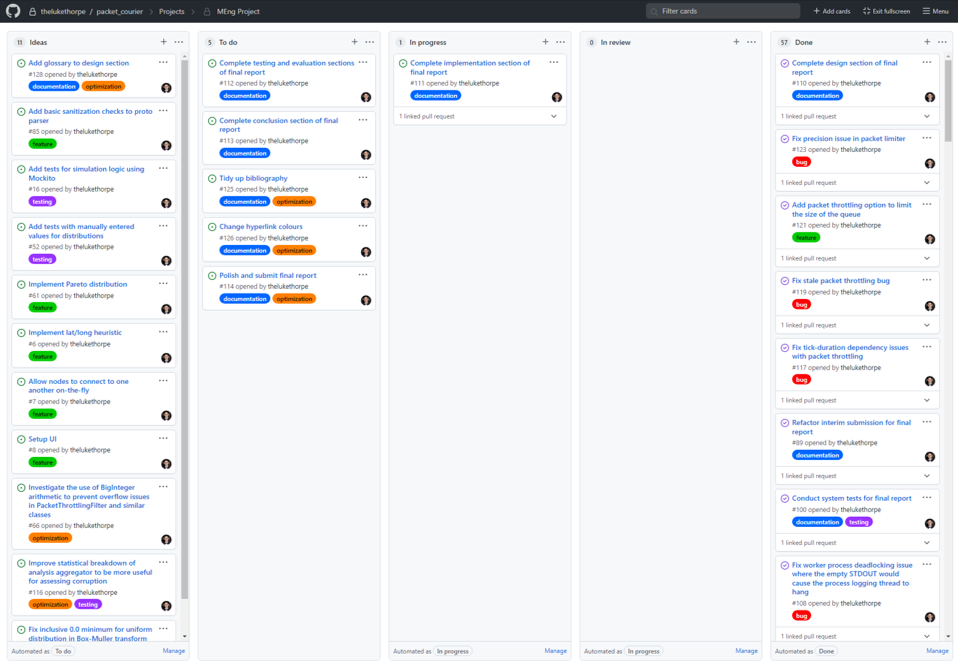
\includegraphics[width=\textwidth]{images/chapter_4_implementation/github_kanban_board}
    \centering~\caption{Packet Courier's Project Kanban Board\cite{packet_courier}.}
    \label{fig:chapter_4_implementation-github_kanban_board}
\end{figure}

Pull-requests are opened for every merge to the \texttt{main} branch and linked to the associated ticket number.
Branches are named with a uniform and consistent structure, prefixed by the issue number followed by a brief subtitle
of the ticket delimited by hyphens. Despite being an individual project, this repository has been maintained to
industry standards of software engineering practices for organisational reasons, and has in turn benefited massively
from it.

\begin{figure}[!h]
    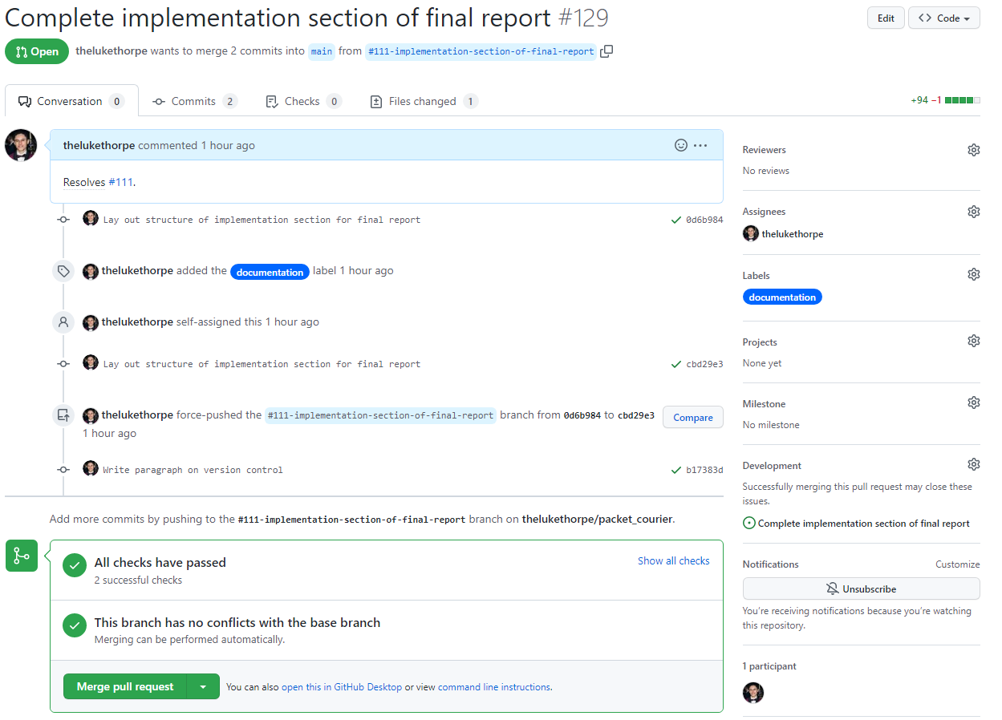
\includegraphics[width=\textwidth]{images/chapter_4_implementation/github_pull_request}
    \centering~\caption{An example of a pull-request in the Packet Courier repository\cite{packet_courier}.}
    \label{fig:chapter_4_implementation-github_pull_request}
\end{figure}

\newpage

\subsection{Programming Languages}

Java 8\cite{java_8} was chosen as the foundational language for Packet Courier due to:
\begin{itemize}
    \item Its excellent breadth of supported platforms\cite{java_8_support}, which lends itself well to objective 4.a).
    \item The vast number of popular and easily importable libraries available to it\cite{java_relevance}.
    \item Its object-oriented nature, which maps nicely onto the abstract semantics laid out in the design section.
    \item Its relatively high levels of time-efficiency, as shown in
    Figure~\ref{fig:chapter_4_implementation-programming_language_comparison}.
    \item Its suite of concurrency abstractions\cite{java_util_concurrent}.
\end{itemize}

\begin{figure}[!h]
    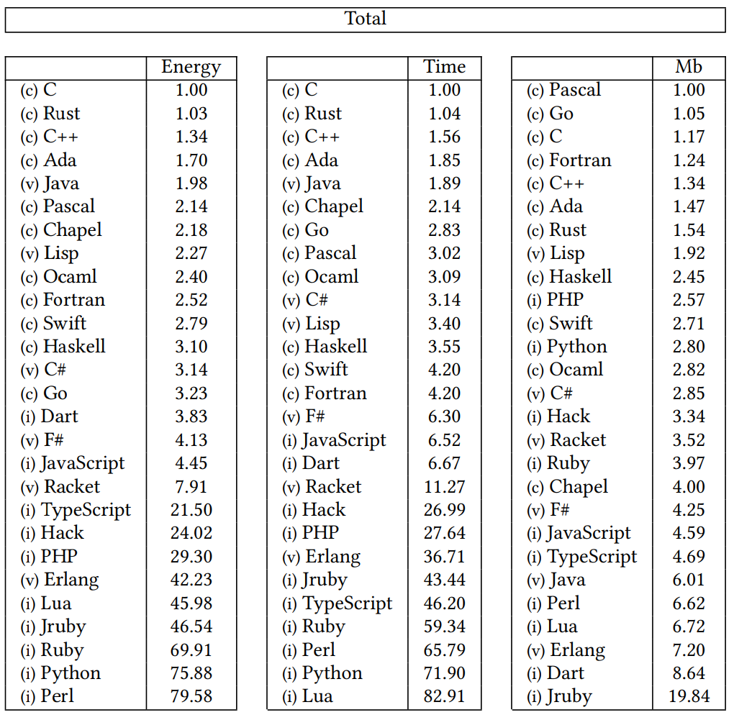
\includegraphics[width=\textwidth]{images/chapter_4_implementation/programming_language_comparison}
    \centering~\caption{A comparison of programming languages based on energy usage, time and memory
    efficiency\cite{programming_language_efficiency}.}
    \label{fig:chapter_4_implementation-programming_language_comparison}
\end{figure}

Although languages such as C and C++ outperform Java across all metrics displayed by
Figure~\ref{fig:chapter_4_implementation-programming_language_comparison}, they are needlessly low-level to the point
where it would likely become a hindrance. Even a cursory investigation into the nature of socket programming in C++
revealed a perfect case study as to the benefits of Java for a problem statement like Packet Courier's. It turns out
that Windows does not natively support the standard C++ socket specification, \texttt{sys/socket.h}, meaning that
\texttt{winsock2.h} must be used instead\cite{socket_vs_winsock}. This would then mean either going to the effort of
implementing two different platform-dependent solutions, or using a library that promises platform agnosticism. There
are many such libraries however\cite{c++_socket_libraries}, placing a substantial research burden on the development
of what should be a fairly simple component. C++ furthermore has been shown to have several non-trivial cross-platform
and cross-compiler discrepancies for even the most basic code\cite{c++_cross_compiler_differences,
    c++_statistical_differences, c++_random_differences, c++_filesystem_differences}.

A key benefit of Java is that it smooths out cross-platform issues, providing developers with a clean, uniform and
highly reliable set of semantics that transcend the nuances of the native operating system and hardware
micro-architecture. Indeed, Java handily has a \texttt{DatagramSocket} class\cite{java_DatagramSocket} which has
proven extremely useful in implementing Packet Courier's standalone emulator. In this way, external Java libraries
are only called-in for more heavyweight or highly specific work, as opposed to routine or menial implementations.

Java also strikes a Goldilocks-esque balance\cite{goldilocks_effect} between low-level languages like C++ and
languages that are arguably even more abstract than Java, such as Python. Whilst Packet Courier does leverage Python
3\cite{python_3} for basic client-server scripts to demonstrate the functionality of the emulator, production code
consists exclusively of Java. Python's dynamic typing\cite{python_typing}, poor
performance\cite{programming_language_efficiency} and inefficient multi-threading and synchronisation
primitives\cite{python_gil} are the main reasons why it wasn't used more prominently within Packet Courier.

\subsection{Build and Dependency Management}

Packet Courier uses Apache Maven 3.6.3\cite{maven} to manage its build phases and dependencies. Maven is convienent,
lightweight, widely supported, boasts a huge repository of libraries\cite{maven_repository} and with a single
command can compile the project into a portable \texttt{.jar} file that can be used as an executable binary or a Java
library.

\subsubsection{JUnit 4}

JUnit 4\cite{juint4} is an industry standard for conducting tests in Java, with an estimated 30.7\% of Java projects on
GitHub using JUnit (according to a study done in 2013)\cite{java_library_popularity}. Naturally, the Packet Courier
unit tests are implemented using JUint 4.13 and are run on each Maven build.

\subsubsection{AssertJ}

\begin{lstlisting}[language=Java,caption={An example of a Packet Courier unit test using JUnit and AssertJ.},
    label={code:packet_test},captionpos=b]
public class PacketTest {
  // JUnit 4 test.
  @Test
  public void testPacketStringConversion() {
    String message = "hello there!";
    Packet messageAsPacket = Packet.of(message);
    // AssertJ assertion reads like an English sentence.
    assertThat(messageAsPacket.tryParse()).hasValue(message);
  }

  // Some more tests...
}
\end{lstlisting}


AssertJ\cite{assert_j} is used in conjunction with JUnit to provide unit tests with expressive, human-readable checks
as shown in Code-Snippet~\ref{code:packet_test}. The following paragraph from a \emph{JavaZone} article summarises
why AssertJ was favoured over the JUnit default assertion framework known as Hamcrest\cite{assert_j_vs_hamcrest}:
\begin{quote}
    \emph{``AssertJ is not as well-known as Hamcrest, but at the same time, its popularity has been growing pretty
    fast over the last few years. As opposed to Hamcrest’s classic assertion syntax, which was inherited from the
    default Java testing framework JUnit, the main idea of AssertJ is that it provides fluent syntax. The main goal
    of that is to improve code readability. It’s worth mentioning that AssertJ is a fork of the FEST Assert project,
        which was the first step of AssertJ creation.''}
\end{quote}

\subsubsection{Google Protocol Buffer}

Google Protocol Buffer\cite{google_protobuf} is a multi-faceted library that is supported across multiple languages,
but is used by Packet Courier to parse configuration files into Java objects. There are many file parsing libraries
for specific file formats, such as Google Gson, a Java JSON parsing library\cite{google_gson}. The unique selling
point of Google Protocol Buffer is its neatly compartmentalised workflow:
\begin{enumerate}
    \item Write a \texttt{.proto} file that defines the expected file structure. See
    Code-Snippet~\ref{code:google_protocol_buffer_example} for an example.
    \item Compile the \texttt{.proto} file using Maven to generate the corresponding parse-tree in Java.
    \item Choose a parser such as \texttt{JsonFormat} to generate a parse-tree from an input file.
    \item Perform a semantic pass over the parse-tree, i.e.: completing basic sanity checks whilst converting the
    raw syntactic form of the parse-tree into something more abstract that can be assimilated into the core APIs.
\end{enumerate}

\begin{lstlisting}[language=protobuf2,style=protobuf,caption={An example of a \texttt{.proto} file that encodes for
an \texttt{AddressBook}. A data file that followed this syntactic structure could then be read into memory as an
\texttt{AddressBookProtos} Java class, ready for further abstraction.},
    label={code:google_protocol_buffer_example},captionpos=b]
    syntax = "proto2";

    package tutorial;

    option java_multiple_files = true;
    option java_package = "com.example.tutorial.protos";
    option java_outer_classname = "AddressBookProtos";

    message Person {
        optional string name = 1;
        optional int32 id = 2;
        optional string email = 3;

        enum PhoneType {
            MOBILE = 0;
            HOME = 1;
            WORK = 2;
        }

        message PhoneNumber {
            optional string number = 1;
            optional PhoneType type = 2 [default = HOME];
        }

        repeated PhoneNumber phones = 4;
    }

    message AddressBook {
        repeated Person people = 1;
    }
\end{lstlisting}

\subsubsection{Protocol Buffers Protobuf Maven Plugin}

An unusual quirk of the Google Protocol Buffer Java library is that it doesn't compile all of the requisite Java
classes into the final \texttt{.jar}; instead it assumes that they will be loaded into the project as part of a
separate library. The \texttt{protoc-jar-maven-plugin}\cite{protoc_jar_maven_plugin} helps to work around this issue
by adding an extra compilation step at compile time to plug this gap.

\subsection{Continuous Integration}

The Packet Courier repository uses GitHub actions\cite{github_actions} to implement a continuous integration
pipeline\cite{aws_ci} where code is linted and tested, both of which are done using Maven. Linting is enforced using
\texttt{fmt-maven-plugin}\cite{fmt_maven_plugin}, which provides users with an automated way to check for and fix Java
code that does not adhere to the Google Java Style Guide\cite{google_java_format, google_java_style_guide}. Testing
is simply done via the Maven command:
\begin{quote}
    \texttt{mvn '-Dtest=**.*Test' test --no-transfer-progress}.
\end{quote}


\newpage


\section{API Overview}

\subsection{Repository Structure}

\begin{figure}[!h]
    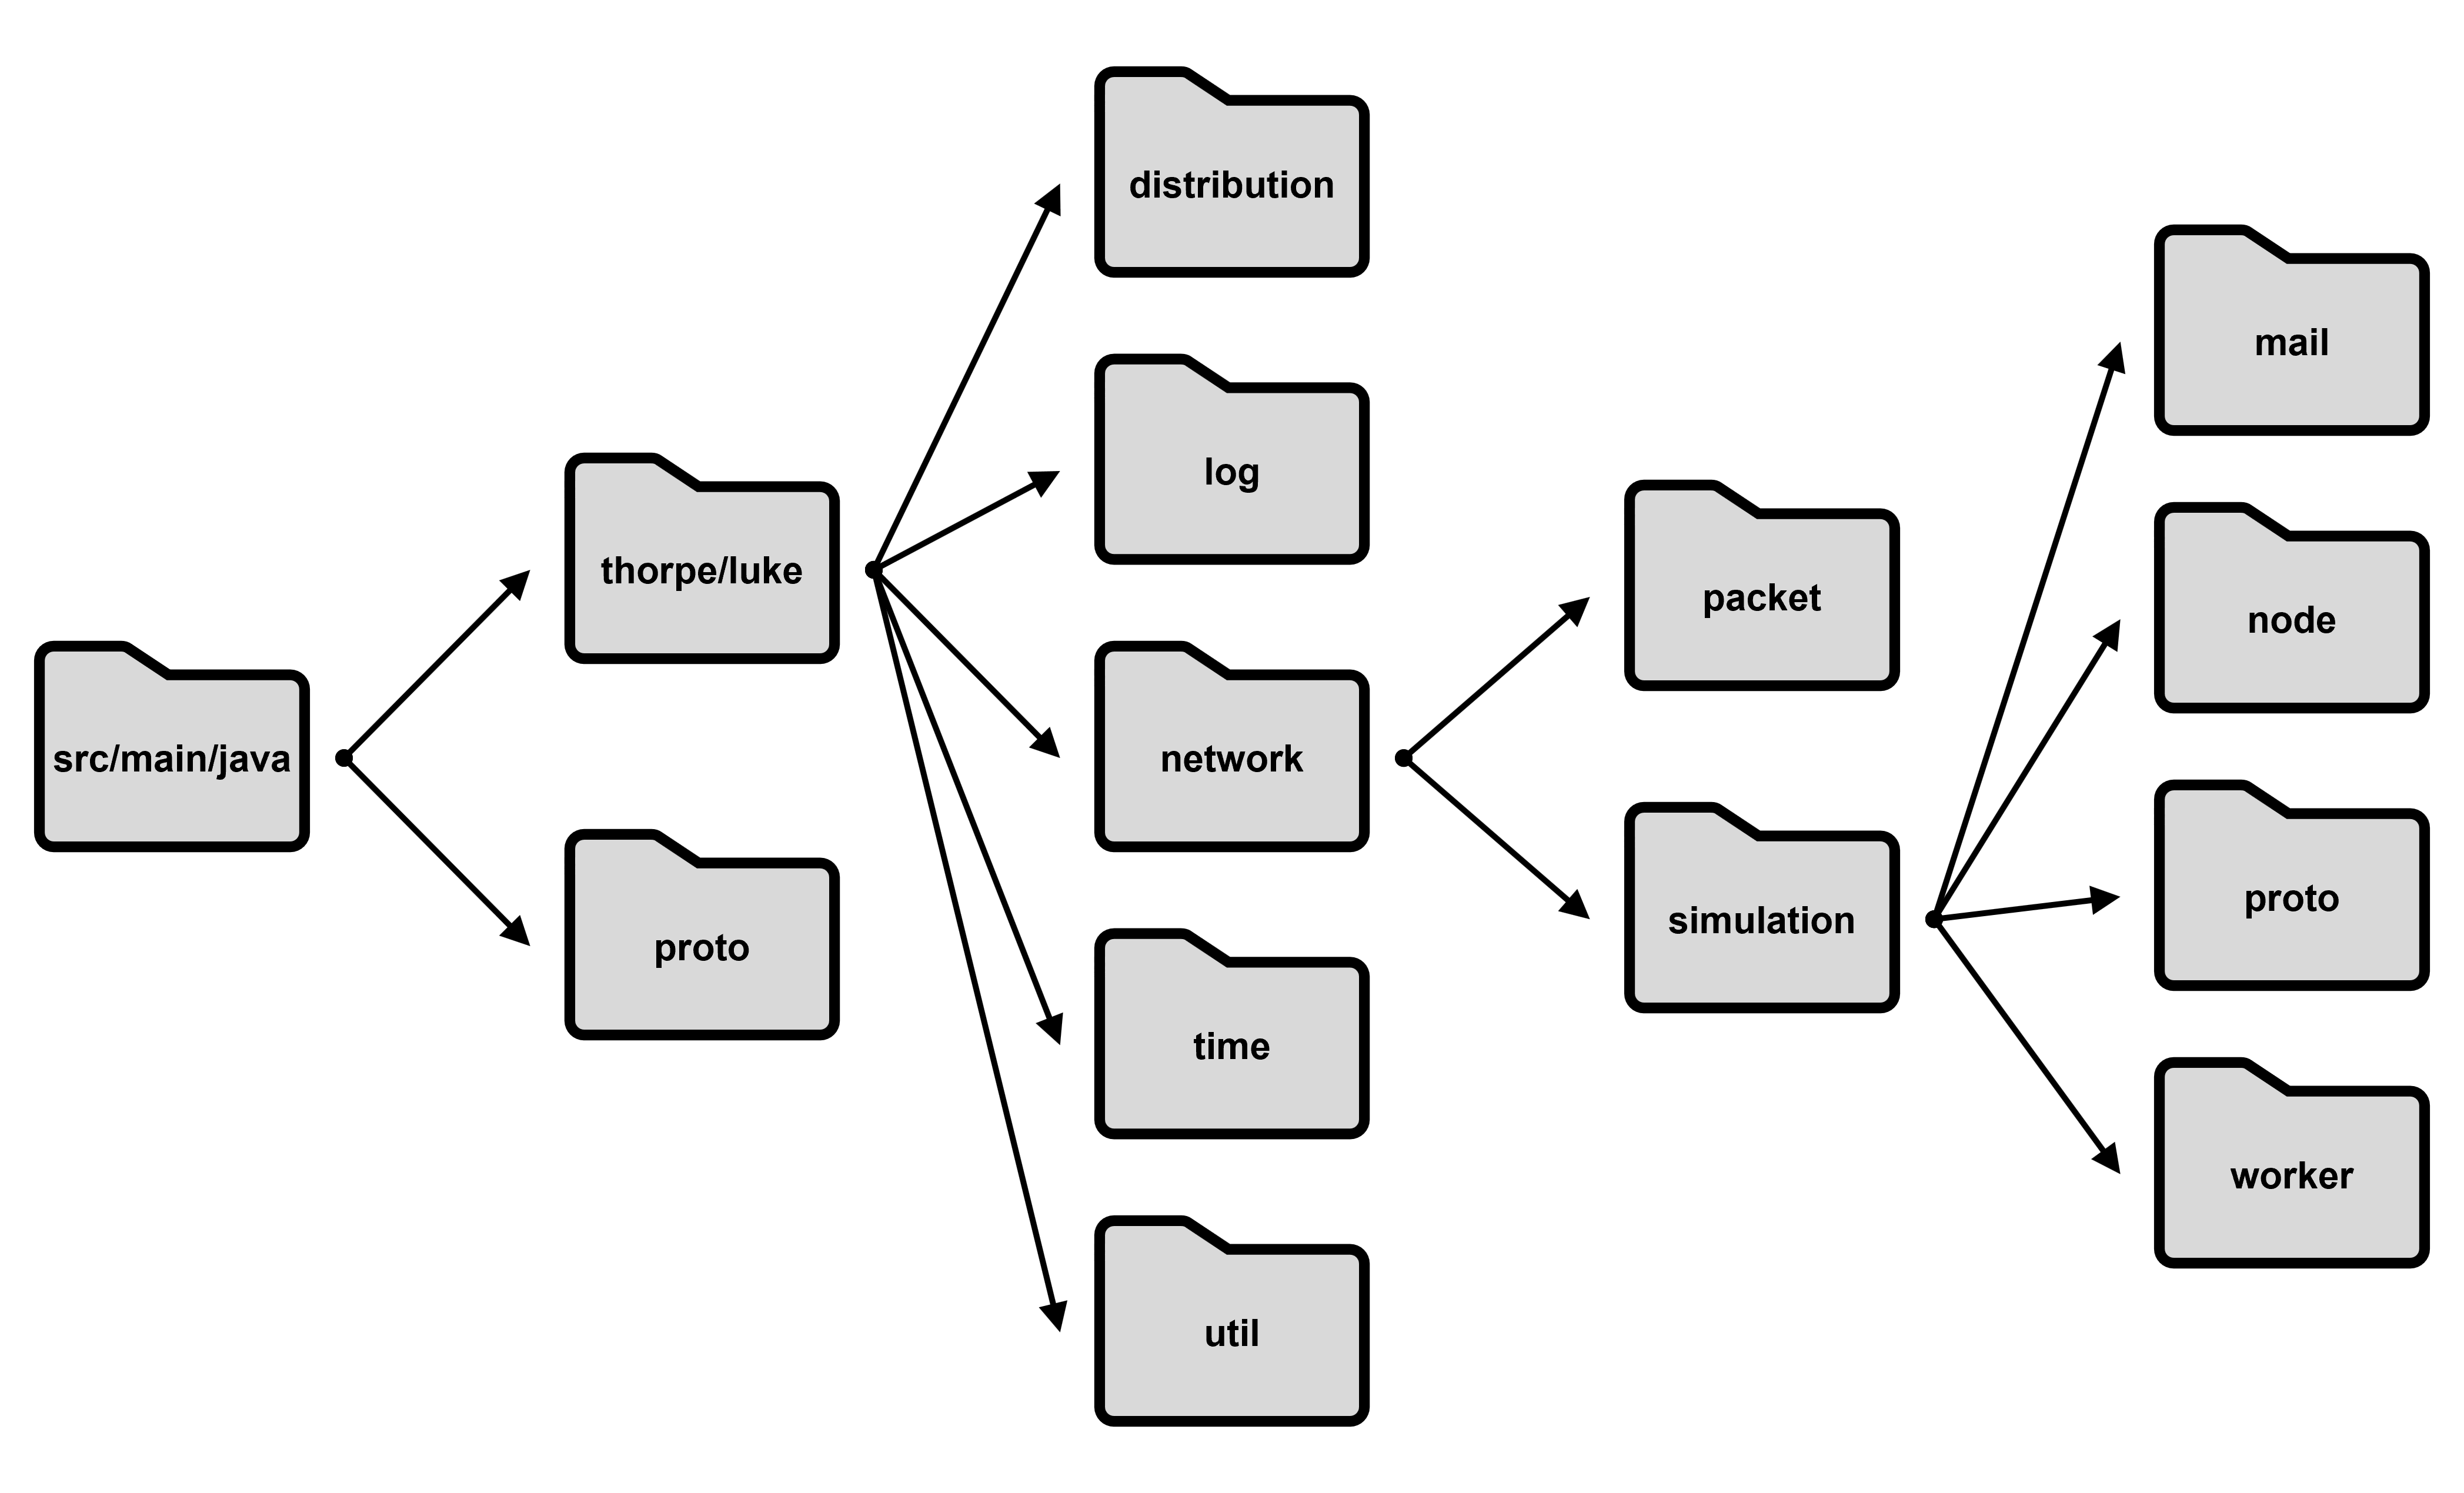
\includegraphics[width=\textwidth]{images/chapter_4_implementation/repository_structure}
    \centering~\caption{A diagram showing the directory tree of the repository's source code. The tests reside in
    \texttt{src/test} and are analogously structured.}
    \label{fig:chapter_4_implementation-repository_structure}
\end{figure}

\subsection{Statistical Distribution API}

Packet Courier supports the following statistical distributions:
\begin{itemize}
    \item Bernoulli
    \item Exponential
    \item Normal
    \item Poisson
    \item Continuous (Real) Uniform
    \item Discrete (Integer) Uniform
\end{itemize}

Each distribution implementation implements the \texttt{Distribution<T>} interface as shown in
Figure~\ref{fig:chapter_4_implementation-distribution_api_tree}, whereby type parameter \texttt{T} corresponds to the
type of value returned by the sampling function.

\begin{figure}[!h]
    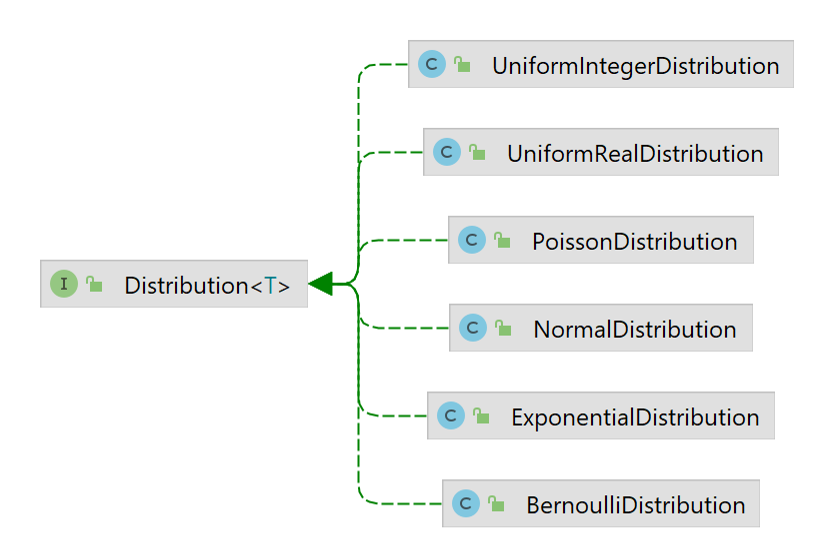
\includegraphics[width=0.65\textwidth]{images/chapter_4_implementation/distribution_api_tree}
    \centering~\caption{A diagram showing the class inheritance tree of the distribution API.}
    \label{fig:chapter_4_implementation-distribution_api_tree}
\end{figure}

As per Code-Snippet~\ref{code:distribution_inferface}, Packet Courier distributions adhere to the C++
distribution-generator pattern where the source of randomness, or \emph{generator}, is decoupled from the
parameterised statistical distribution that is being sampled from\cite{c++_random, c++_random_number_generation}. In
addition to the fact that decoupling is generally a good programming practice\cite{decoupling}, there are several
application-specific benefits to separating a distribution from its sampling
engine\cite{c++_random_number_generation_philosophy}:
\begin{itemize}
    \item Distributions are far more lightweight when they don't need to carry around a source of randomness. Indeed,
    there are a number of places within the Packet Courier codebase that create a temporary distribution to be
    sampled on-the-fly, as demonstrated in Code-Snippet~\ref{code:sample_from_event_duration_distribution}. If the
    distribution needed to be created with a source of randomness ahead of time, then this would likely result in
    much clumsier code. Of course, \texttt{Random} could be passed in as a constructor parameter, which wouldn't
    affect Code-Snippet~\ref{code:sample_from_event_duration_distribution} in any way, but it would make the
    distribution stateful.
    \item Stateful distributions are less useful and needlessly more prone to error. Indeed, a stateless distribution
    with no embedded source of randomness can be used in multiple different contexts or even across different
    threads. Consider a scenario where a Poisson distribution is being used to model the number of sheep in a field.
    Suppose a developer wanted to conduct two simulations for the same value of $\lambda$: one with pure randomness
    and the other with a correlation bias. Decoupling means that the same distribution can be used to conduct both
    experiments in parallel, whereas two of the same distribution would need to be created if the generator were
    embedded in the distribution. Indeed, this is especially suboptiomal in the case of a Poisson distribution,
    since the Packet Courier implementation generates a table for each distribution.
    \item Depending on how deeply embedded the random number generation engine is in the distribution, it could
    result in correlated results. For example, if two different normal distributions used a common seed for two
    different instances of \texttt{Random}, then the same sequence would be generated. As a consequence, the
    Box-Muller transform would generate the same values of $Z \sim \mathcal{N}(0,1)$\cite{box_muller_transform}. Even
    if the two distributions were parameterised differently, the two output sequences would still be linear functions
    of one another since $Z \sim \mathcal{N}(0,1) \implies \mu + \sigma Z \sim \mathcal{N}(\mu, \sigma^2)$. One might
    argue that this could be resolved by using different seeds for each distribution; notice that this becomes a
    nightmare very quickly, i.e.: coordinating the unique usage of seeds across all distributions, especially if
    seeds are user-parameterised. The much simpler solution is just to decouple random generation from
    stateless distributions.
\end{itemize}

\begin{lstlisting}[language=Java,caption={The \texttt{Distribution<T>} interface exactly as it appears in the
codebase.},label={code:distribution_inferface},captionpos=b]
public interface Distribution<T> {
  T sample(Random random);

  Double mean();

  Double variance();
}
\end{lstlisting}

\begin{lstlisting}[language=Java,caption={An example of a distribution being created and sampled on-the-fly with
arbitrary parameters.},label={code:sample_from_event_duration_distribution},captionpos=b]
public class SimulatedEventPipeline<Wrapper extends PacketWrapper<Wrapper>> implements PacketFilter<Wrapper> {
  // Random generator.
  private final Random random;

  // Method that generates the duration of a particular event,
  // as per the event-based semantics.
  private LocalDateTime sampleFromEventDurationDistribution(double meanDuration) {
    // Distribution is generated on-the-fly and used with
    // the class's in-house source of randomness.
    ExponentialDistribution eventDurationDistribution =
        new ExponentialDistribution(1.0 / meanDuration);
    long eventDuration = Math.round(eventDurationDistribution.sample(random));
    return now.plus(Duration.of(eventDuration, timeUnit));
  }

  // Rest of class...
}
\end{lstlisting}

Classes inheriting from \texttt{Distribution<T>} must also implement the \texttt{mean} and \texttt{variance} methods
for testing purposes. This will be discussed in more detail later in the report, but in short, both statistics are
required to compute a confidence interval\cite{confidence_interval}.


\newpage

\subsection{Network Condition API}

\begin{figure}[!h]
    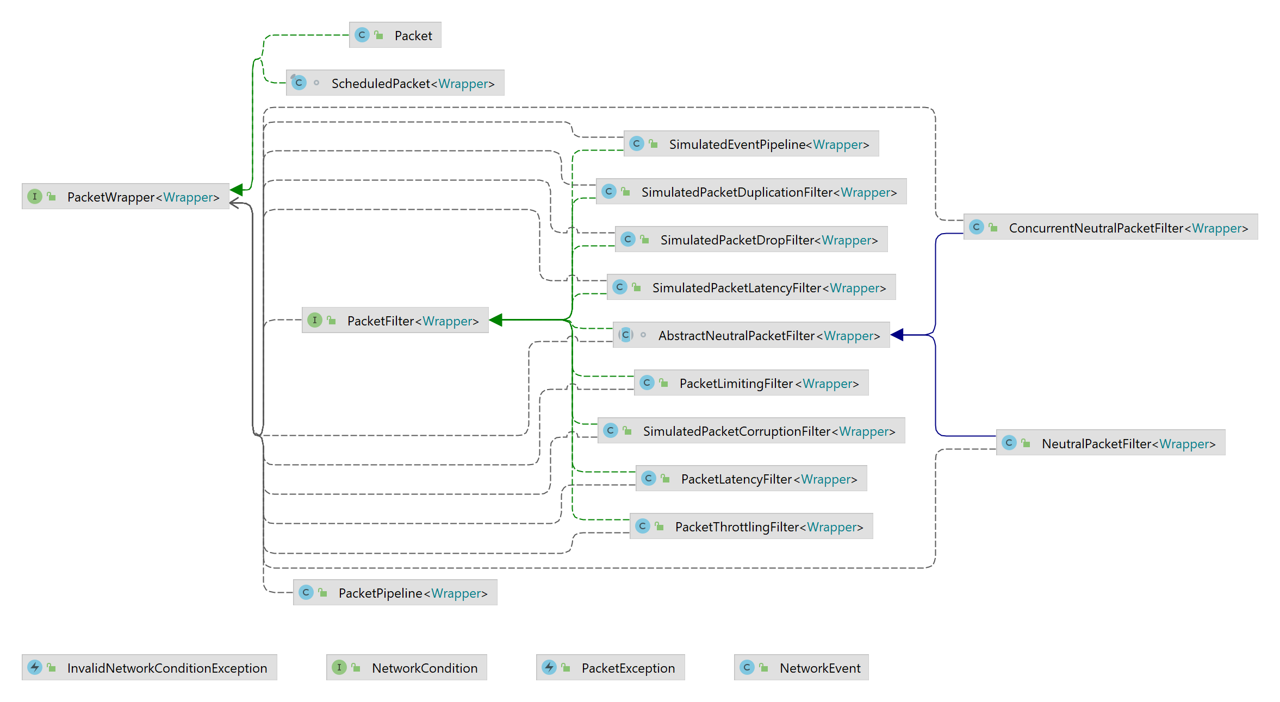
\includegraphics[width=0.8\textwidth]{images/chapter_4_implementation/network_condition_api_tree}
    \centering~\caption{A diagram showing the class inheritance tree of the network condition API.}
    \label{fig:chapter_4_implementation-network_condition_api_tree}
\end{figure}

\subsubsection{Packet \& PacketWrapper}

The \texttt{Packet} class is, by and large, the atomic building block for Packet Courier, despite only being a humble
wrapper for a list of bytes. A flagship feature of \texttt{Packet} is its ability to transform freely from a Java
object and back again, as demonstrated in Code-Snippet~\ref{code:packet_test}. This is achieved using Java's
\texttt{Serializable} interface\cite{java_Serializable}, which imbues inheriting classes with a canonical
representation at the level of bits; a crucial factor for communication over a wire. Furthermore, the JVM handles
serialization under-the-hood, so all a programmer needs to do is write \texttt{implements Serializable} after the
definition of a class they wish to be mailed as a \texttt{Packet}. For example, if a Packet Courier user were
simulating an authentication process using a custom class named \texttt{UserCredentials} with two \texttt{String}
attributes, \texttt{username} and \texttt{password}, then \texttt{UserCredentials} objects could be sent from worker
to worker so long as the \texttt{Serializable} interface was implemented.

\texttt{Packet} inherits from \texttt{PacketWrapper<Packet>}, a type-parameterised interface defined as follows:

\begin{lstlisting}[language=Java,caption={The \texttt{PacketWrapper<Wrapper>} interface exactly as it appears in the
codebase.},label={code:packet_wrapper_interface},captionpos=b]
public interface PacketWrapper<Wrapper extends PacketWrapper<Wrapper>> {
  Wrapper map(Function<Packet, Packet> function);

  Wrapper copy();

  Packet getPacket();
}
\end{lstlisting}


\texttt{PacketWrapper<Wrapper>} allows non-packet objects to be sent through packet pipelines. The motivation behind
this is simple: packet pipelines deal in terms of \emph{packets} and nothing else, yet there are plenty of scenarios
where users of the API might want to their packets to carry additional information as they travel through a pipeline.
The principle example within the wider context of Packet Courier is the \texttt{Mail} class, which holds the packet's
destination address for routing purposes. However, \texttt{PacketWrapper<Wrapper>} could also be used for telemetry,
instrumentation, timestamping and other broader logging purposes; any important meta-information about the packet
that users of the API might find useful.

The semantics of the \texttt{PacketWrapper<Wrapper>} interface can be likened to those of functional
homogeneity\cite{homogeneous_function}. Classes that implement \texttt{PacketWrapper<Wrapper>} provide external code
with the means to manipulate the \texttt{Packet} residing inside the wrapper without interacting with any other
aspect of the object; a similar sentiment to keyhole surgery\cite{keyhole_surgery}.

An arguably simpler solution is to use inheritance rather than composition, whereby \texttt{Mail}, say, inherits from
\texttt{Packet} and is sent through the pipeline before being cast back to \texttt{Mail} having emerged on the other
side. This is majorly inferior for many reasons:
\begin{itemize}
    \item This approach would be considered a ``hack'', since it does not make idiomatic sense within the context of
    Java. Given that \texttt{Mail} would inherit from \texttt{Packet}, then one would conclude that \texttt{Mail}
    \emph{is} a kind of \texttt{Packet}. This is not true though, in the same way that a letter isn't a type of
    envelope, but is contained within one. Indeed, as per the semantics laid out in the design document,
    \texttt{Mail} \emph{has} a \texttt{Packet}, and therefore composition is more appropriate.
    \item Casting in this way is widely agreed upon by Java programmers to be a poor practice, with excellent reasons
    to back this up\cite{reddit_casting, yegor_bugayenko_casting, mark_casting, dennis_sosnoski_casting,
        erik_dietrich_casting}.
    \item There are practical limitations to this method as well. How would more invasive packet manipulations such
    as corruption and duplication work whilst still preserving the outer class? It \emph{could} be done using
    methods such as \texttt{clone}\cite{java_clone}, but it would ultimately result in more convoluted and fragile
    code\cite{java_avoid_clone}.
\end{itemize}

\subsubsection{PacketFilter \& PacketPipeline}

The \texttt{PacketFilter<Wrapper>} interface represents a single step in a packet pipeline and is defined as follows:
\begin{lstlisting}[language=Java,caption={The \texttt{PacketFilter<Wrapper>} interface exactly as it appears in the
codebase.},label={code:packet_filter_interface},captionpos=b]
public interface PacketFilter<Wrapper extends PacketWrapper<Wrapper>> {
  void tick(LocalDateTime now);

  void enqueue(Wrapper packetWrapper);

  Optional<Wrapper> tryDequeue();
}
\end{lstlisting}

A \texttt{PacketFilter<Wrapper>} can be conceptualised as a queue of packets that admits of special behaviour and can
be synced up with the wider simulation using the \texttt{tick} method. For example, the
\texttt{SimulatedPacketDropFilter<Wrapper>} will sample its Bernoulli distribution whenever the \texttt{enqueue}
method is called, whereby the packet is never actually enqueued if the sample is ``successful''. Another example is
the \texttt{PacketLatencyFilter<Wrapper>}\footnote{Packet filters prefixed with \texttt{Simulated} have some kind of
random component to them; conversely, filters without this prefix are deterministic and provide what could in
principle be real-world utility, such as packet throttling.} which takes instances of
\texttt{ScheduledPacket<Wrapper>} as the parameter for its \texttt{enqueue} method and stores them in a priority
queue with the packet scheduled for dequeue at the earliest time at the front of the queue. In turn,
\texttt{tryDequeue} will only release the packet at the front of the queue if a) it exists, b) its scheduled dequeue
time has passed with respect to the current simulation time; indeed, the purpose of \texttt{tick} here is to
synchronise the filter with the simulation's clock. The \texttt{NeutralPacketFilter<Wrapper>} is a simple filter with
FIFO semantics with the \texttt{ConcurrentNeutralPacketFilter<Wrapper>} being its thread-safe counterpart.

In this way, the \texttt{enqueue} and \texttt{tryDequeue} methods of packet filters can be chained together to form a
packet pipeline. In fact, this is precisely how the \texttt{PacketPipeline<Wrapper>} class works, as shown in
Code-Snippet~\ref{code:packet_pipeline_class}.
\begin{lstlisting}[language=Java,caption={A cut-down version of the \texttt{PacketPipeline<Wrapper>} class.},
    label={code:packet_pipeline_class},captionpos=b]
public class PacketPipeline<Wrapper extends PacketWrapper<Wrapper>> {
  private final List<PacketFilter<Wrapper>> packetFilters;

  private PacketPipeline(List<PacketFilter<Wrapper>> packetFilters) {
    packetFilters.add(0, new ConcurrentNeutralPacketFilter<>());
    this.packetFilters = Collections.unmodifiableList(new ArrayList<>(packetFilters));
  }

  public void enqueue(Wrapper packetWrapper) {
    packetFilters.get(0).enqueue(packetWrapper);
  }

  public void tick(LocalDateTime now) {
    for (int i = 0; i + 1 < packetFilters.size(); i++) {
      PacketFilter<Wrapper> currentFilter = packetFilters.get(i);
      PacketFilter<Wrapper> nextFilter = packetFilters.get(i + 1);
      currentFilter.tryDequeue().ifPresent(nextFilter::enqueue);
      nextFilter.tick(now);
    }
  }

  public Optional<Wrapper> tryDequeue() {
    PacketFilter<Wrapper> lastFilter = packetFilters.get(packetFilters.size() - 1);
    return lastFilter.tryDequeue();
  }
}
\end{lstlisting}

Each packet pipeline starts off with a \texttt{ConcurrentNeutralPacketFilter<Wrapper>}, not only for algorithmic ease
(i.e.: not having to do an empty check on \texttt{packetFilters} when enqueuing or dequeuing), but to ensure that
enqueuing to a packet pipeline is always a thread-safe operation. This is important because workers do their work in
parallel with one another and thus can send mail along the same channel concurrently. The \texttt{tick} and
\texttt{tryDequeue} methods needn't be thread-safe, however, which will become apparent later in this section when
their use-case is discussed.

Note that \texttt{PacketPipeline<Wrapper>} could in principle inherit from \texttt{PacketFilter<Wrapper>}, since it
implements the required methods. However, just because one could does not necessarily mean one \emph{should}. In
these circumstances, the purpose of the \texttt{PacketFilter<Wrapper>} interface is to provide developers with an API
to create and use steps in a \texttt{PacketPipeline<Wrapper>}. How would making \texttt{PacketPipeline<Wrapper>}
implement \texttt{PacketFilter<Wrapper>} be commencerate with this notion? It would enable programmers to make a
packet pipeline a step in a packet pipeline. Naturally this is a redundant and confusing API behaviour that would
only create potential for bad code.

\subsubsection{NetworkConditions}

The \texttt{NetworkCondition} interface acts as a \texttt{PacketFilter<Wrapper>} factory. It is important that API
users are not given the autonomy to create packet pipelines manually from packet filters or else they risk
experiencing crippling side effects. For example, a developer might decide to ``reuse'' a packet filter for two
different pipelines because the parameters are the same. This would be absolutely disasterous since packets from two
different pipelines would be routed through the \emph{same} filter, coupling them by accident and resulting in packets
going to the wrong workers. To guard against this, the only public \texttt{PacketPipeline<Wrapper>} constructor takes
an instance of the \texttt{PacketPipeline.Parameters} inner class, which is in turn a wrapper for a list of
\texttt{NetworkCondition} objects. This forces API users to create packet pipelines using abstract parameters rather
than straight from filters, delegating the creation of the actual filter instances to the pipeline itself.
\begin{lstlisting}[language=Java,caption={The \texttt{NetworkCondition} interface without any of its presets.},
    label={code:network_condition_interface},captionpos=b]
public interface NetworkCondition {
  <Wrapper extends PacketWrapper<Wrapper>> PacketFilter<Wrapper> asPacketFilterStartingAt(LocalDateTime startTime);
}
\end{lstlisting}

The \texttt{NetworkCondition} interface comes with a suite of static methods that predefine a selection of network
conditions that reflect the packet filtration mechanisms that are outlined by Packet Courier's semantics, including,
but not limited to:
\begin{itemize}
    \item \texttt{static NetworkCondition packetLimit(int packetLimitRate, ChronoUnit timeUnit)}
    \item \texttt{static NetworkCondition uniformPacketCorruption(double corruptionProbability, Random random)}
    \item \texttt{static NetworkCondition normalPacketLatency(double meanLatency, double standardDeviation,
        ChronoUnit timeUnit, Random random)}
\end{itemize}

\subsection{Worker API}

TODO

\subsection{Node API}

TODO

\subsection{Mail API}

TODO

\subsection{Simulation API}

TODO

\subsection{Miscilaneous}

TODO


\section{Standalone Emulator}

\subsection{Key Components}

TODO

\subsection{Protobuf Integration}

TODO


\section{Debugging Features}

\subsection{Process Monitor}

TODO

\subsection{Crash Dumps}

TODO

\subsection{Meta Logging}

TODO
